\documentclass{beamer}
\usetheme{Antibes}

\usepackage{amsfonts}
\usepackage{amssymb}
\usepackage{amsmath}
\usepackage{amsthm}

% My commands
\newcommand{\R}{\mathbb{R}}
\newcommand{\N}{\mathbb{N}}
\newcommand{\Z}{\mathbb{Z}}
\newcommand{\T}{\mathrm{T}}
\newcommand{\E}{\mathbb{E}}
\newcommand{\Var}{\mathrm{Var}}
\newcommand{\Cov}{\mathrm{Cov}}
\newcommand{\Dcal}{\mathcal{D}}

\newtheorem{proposition}{Proposition}

\title[Decision-dependent DRO]{
	Decision-dependent Distributionally Robust Optimization
}
\subtitle{
	The Facility Location Problem with Random Demand
}
\author[Fortin-Leblanc, Joshaghani]{
	Gabriel Fortin-Leblanc\inst{1} \and Mohammad Joshaghani\inst{2}
}
\institute{
	\inst{1}
	Université de Montréal
	\and
	\inst{2}
	Université du Québec à Montréal
}
\date{November 29, 2024}

\begin{document}

\frame{\titlepage}

\begin{frame}{Outline}
	\tableofcontents
\end{frame}

\section{Introduction to the problem} % Gabriel ~ 3 min.
\begin{frame}[allowframebreaks]
	\begin{columns}
		\column{0.4\textwidth}
		\begin{itemize}
			\item Different capacities
			\item Different opening costs
			\item Transportation fees
			\item Opened facilities affect the demand
		\end{itemize}
		Which facilities to open so the cost is minimized?
		
		\column{0.7\textwidth}
		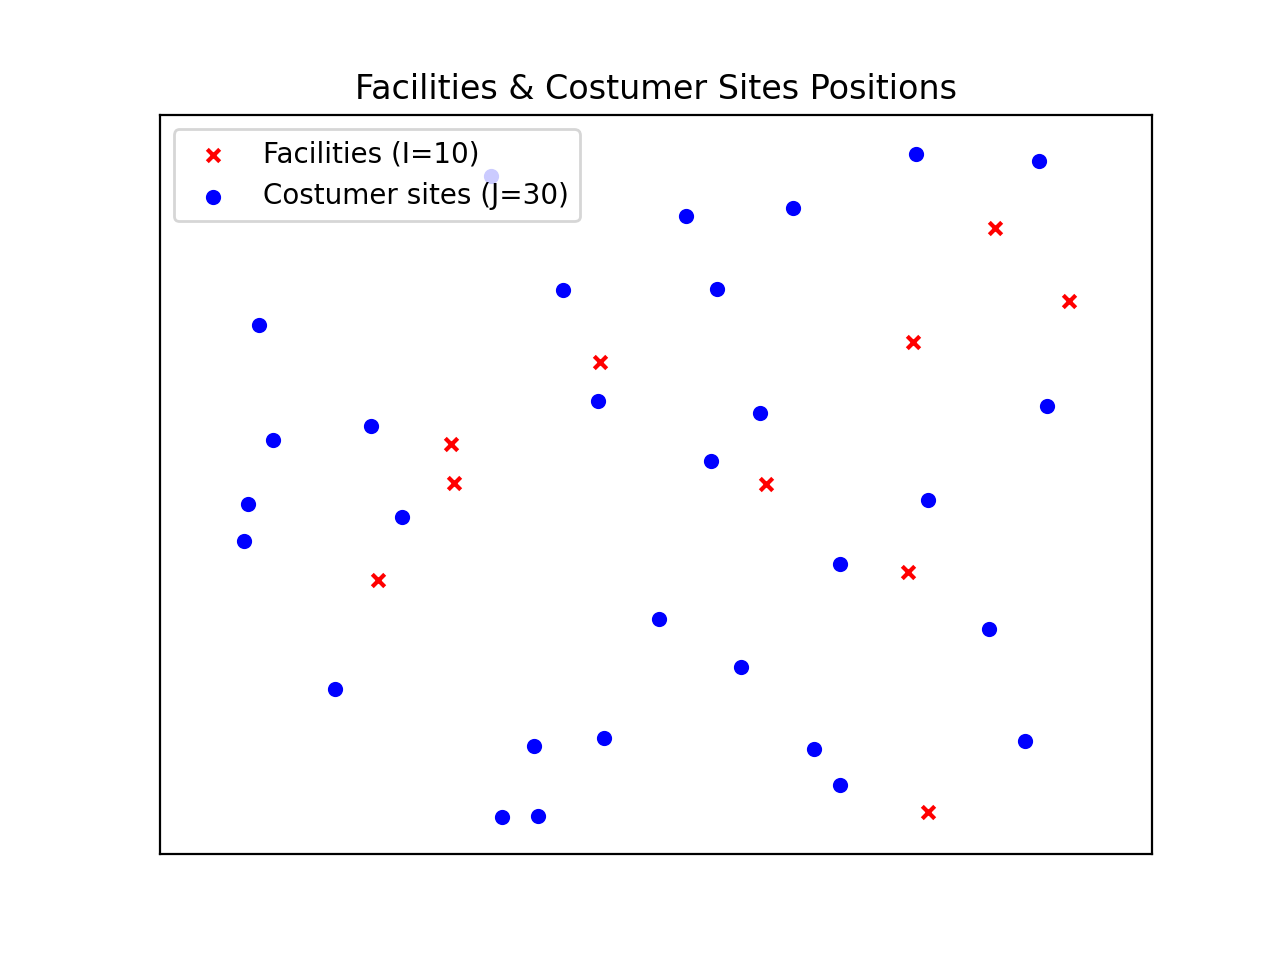
\includegraphics[width=\textwidth]{../figure/facility_costumer_site_pos.png}
	\end{columns}
	
	\framebreak
	\begin{itemize}
		\item $J$ costumer sites
		\item $I$ possible location for facilities
		\item $y \in \{0, 1\}^I$ the decision variables
		\item $O \in \R_+^{I}$ the opening costs
		\item $C \in \R_+^{I}$ the capacities
		\item $t \in \R_+^{I \times J}$ the transportation fees
		\item $\Dcal = \{\xi_k \in \R_+: k \in [K]\}$ the support of the demand (same for each costumer sites)
		\item $d(y) \in \Dcal^J$ the random demand
		\item $r \in \R_+^{J}$ the revenues
		\item $p \in \R_+^{J}$ the penalty for not responding to the demand
	\end{itemize}
\end{frame}

\subsection{Determistic Problem}
\begin{frame}[allowframebreaks]
	The non-robust problem is represented by
	\begin{subequations}
		\begin{align*}
			\min_{y \in \{0, 1\}^{I}} &\quad O^\T y + \sum_{i \in [I]} \sum_{j \in [J]} (t_{ij} - r_j) x_{ij} \\
			\text{s.t.} &\quad \sum_{j \in [J]} x_{ij} \le C_i y_i, \forall i \in [I]\\
			&\quad \sum_{i \in [I]} x_{ij} \le \max\{\Dcal\}, \forall j \in [J] \\
			&\quad x_{ij} \ge 0, \forall i \in [I], j \in [J].
		\end{align*}
	\end{subequations}
\end{frame}	

\subsection{Determistic Problem}
\begin{frame}[allowframebreaks]	
	\centering
	\underline{Issues}
	\begin{itemize}
		\item Assume that costumer sites sell everything they receive.\footnote{\tiny Shehadeh, K.S. and Sanci, E., 2021. Distributionally robust facility location with bimodal random demand. Computers \& Operations Research, 134, p.105257.} 
		\item Don't consider the affect of opening facilities over the demand.
	\end{itemize}
\end{frame}

\subsection{Robust Counterpart Problem}
\begin{frame}[allowframebreaks]
	\begin{definition}[The model\footnote{\tiny Basciftci, B., Ahmed, S., \& Shen, S. (2021). Distributionally robust facility location problem under decision-dependent stochastic demand. European Journal of Operational Research, 292(2), 548–561. https://doi.org/10.1016/j.ejor.2020.11.002
		}]
		For some value $y \in \{0, 1\}^{I}$, let
		\begin{equation*}
			U(y) \subset \left\{\pi \in \R_+^{J \times K}: \pi 1_K = 1_J\right\}
		\end{equation*}
		be a set of distribution over the demand for each customer sites. The \textbf{robust counterpart of a facility location problem (FLP)} is
		\begin{equation} \label{eq:outterproblem}
			\min_{y \in \{0, 1\}^I} \left\{O^\T y + \max_{\pi \in U(y)} \E h(y, d(y))\right\},
		\end{equation}
	\end{definition}
	
	\framebreak
	\begin{definition}[The model]
		where
		\begin{subequations}
			\label{eq:innerproblem}
			\begin{align}
				h(y, d(y)) = \min_{x, s} &\sum_{i \in [I]} \sum_{j \in [J]} t_{ij}x_{ij} + \sum_{j \in [J]} (p_j s_j - r_j d_j(y)) \\
				\text{s.t.} &\sum_{i \in [I]} x_{ij} + s_j = d_j(y) \quad \forall j \in [J] \\
				&x_{ij} \le C_i y_i \quad \forall i \in [I], j \in [J] \\
				&s_i, x_{ij} \ge 0 \quad \forall i \in [I], j \in [J].
			\end{align}
		\end{subequations}
	\end{definition}
\end{frame}

\begin{frame}[allowframebreaks]
	\begin{definition}[Uncertainty set]
		The uncertainty set is
		\begin{equation*}
			\begin{split}
				U(y) = \left\{\{\pi_j\}_{j \in [J]} \subset \R_+^{K} : \sum_{k=1}^{K} \pi_{jk} = 1, \right.\\
				\left|\E_{\pi_j}[d] - \mu_j(y)\right| < \varepsilon_j^\mu, \\
				\left(\sigma_j^2(y) + (\mu_j(y))^2\right)\underline{\varepsilon}_j^\sigma \le
				\E_{\pi_j}[d^2] \le \left(\sigma_j^2(y) + (\mu_j(y))^2\right)\overline{\varepsilon}_j^\sigma \Bigg\},
			\end{split}
		\end{equation*}
	\end{definition}
	
	\framebreak
	\begin{definition}[Uncertainty set]
		where \footnote{\tiny Shaheen, S. A., Cohen, A. P., \& Roberts, J. D. (2006). Carsharing in North America: Market Growth, Current Developments, and Future Potential. Transportation Research Record, 1986(1), 116–124. https://doi.org/10.1177/0361198106198600115
		\\ Hernández, B., Jiménez, J., \& Martín, M. J. (2010). Customer behavior in electronic commerce: The moderating effect of e-purchasing experience. Advances in Internet Consumer Behavior\& Marketing Strategy, 63(9), 964–971. https://doi.org/10.1016/j.jbusres.2009.01.019
		}
		\begin{align*}
			\mu_j(y) &= \min\left\{\bar{\mu}_j \left(1 + \sum_{i \in [I]} \lambda_{ji}^\mu y_i\right), \mu_j^{\mathrm{UB}}\right\} \\
			\sigma_j^2(y) &= \max\left\{\bar{\sigma}_j^2 \left(1 + \sum_{i \in [I]} \lambda_{ji}^\sigma y_i\right), (\sigma_j^{\mathrm{LB}})^2\right\}.
		\end{align*}
	\end{definition}
\end{frame}

\section{Derive a MILP} % Gabriel ~ 7 min.
\begin{frame}
	\begin{enumerate}
		\item Retrieve a single-level minimization.
		\item Linearize bilinear ($xy$) and trilinear ($xyz$) terms.
	\end{enumerate}
\end{frame}

\subsection{Single-Level Problem}
\begin{frame}[allowframebreaks]
	Steps for obtaining a single-level minimization:
	\begin{enumerate}
		\item Use the duality theorem with the inner Problem \ref{eq:innerproblem} to obtain a maximization problem.
		\item Combine the maximum from the duality to the maximum of the Problem \ref{eq:outterproblem}.
		\item Use the duality theorem with the combined maximization problem to obtain a minimization problem.
	\end{enumerate}
	
	\framebreak
	\begin{proposition}
		The inner Problem \ref{eq:innerproblem} can be computed by
		\begin{equation}
			\label{eq:transformed_h}
			\begin{split}
				h(y, d(y)) = \sum_{j \in [J]} \left(\max_{i' \in \{0, \dots, I\}}\left\{t_{i'j}d_j(y) + \sum_{i \in [I]: t_{ij} < t_{i'j}} C_iy_i(t_{ij} - t_{i'j})\right\}\right.\\ - r_jd_j(y)\Bigg),
			\end{split}
		\end{equation}
		where $t_{0j} = p_j$.
	\end{proposition}
	
	\framebreak
	\underline{Idea of the proof}
	\begin{enumerate}
		\item Separate $h$ into $J$ independent maximization problem
		\item Use the duality theorem
		\item Find by logic the optimal values for the dual variables
	\end{enumerate}
	
	\framebreak
	\begin{theorem}
		The Problem \ref{eq:outterproblem} is equivalent to the single-level minimization given by
		\begin{align*}
			\min_{y, \alpha, \delta^1, \delta^2, \gamma^1, \gamma^2} O^\T y + \sum_{j \in [J]} \Bigg( &\alpha_j + \delta_j^1 \left(\mu_j(y) + \varepsilon_j^\mu\right) - \delta_j^2 \left(\mu_j(y) - \varepsilon_j^\mu\right) \\
			& + \gamma_j^1 \left(\sigma_j^2(y) + (\mu_j(y))^2\right)\overline{\varepsilon}_j^\sigma \\
			& - \gamma_j^2 \left(\sigma_j^2(y) + (\mu_j(y))^2\right)\underline{\varepsilon}_j^\sigma
		\end{align*}
		\begin{align*}
			\text{s.t.}\quad &\alpha_j + (\delta_j^1 - \delta_j^2)\xi_k + (\gamma_j^1 - \gamma_j^2)\xi_k^2 \ge \theta_{jk}(y), \forall j \in [J], k \in [K], \\
			& y \in \{0, 1\}^I, \quad \delta_j^1, \delta_j^2, \gamma_j^1, \gamma_j^2 \ge 0, \forall j \in [J],
		\end{align*}
	\end{theorem}
	
	\framebreak
	\begin{theorem}
		where
		\begin{equation*}
			\theta_{jk}(y) = t_{i^\star j} \xi_k + \sum_{i \in [I]: t_{ij} < t_{i^\star j}} C_i y_i (t_{ij} - t_{i^\star j}) - r_j \xi_k
		\end{equation*}
		with $i^\star$ the index that maximize the problem from Equation \ref{eq:transformed_h}.
	\end{theorem}
\end{frame}

\subsection{Linearized Problem}
\begin{frame}
	\begin{columns}
		\column{0.5\textwidth}
		McCormick envelope\footnotemark[1]
		\begin{itemize}
			\item Gives a ``framework" to replace non linear functions by a variable with constraints
			\item For bilinear terms and trilinear terms, if only one variable is continuous and the others are binary variable, then the problems are equivalent
		\end{itemize}
		
		\column{0.6\textwidth}
		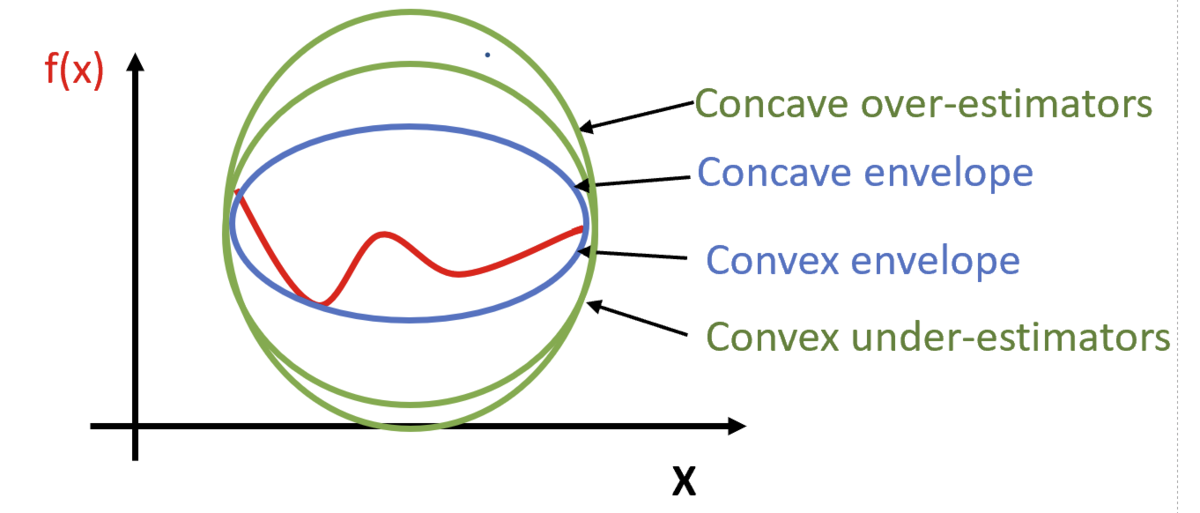
\includegraphics[width=\textwidth]{../figure/mccormick.png}\footnotemark[2]
	\end{columns}
	\footnotetext[1]{McCormick, G. P. (1976). Computability of global solutions to factorable nonconvex programs: Part I — Convex underestimating problems. Mathematical Programming, 10(1), 147–175. https://doi.org/10.1007/BF01580665}
	\footnotetext[2]{https://optimization.cbe.cornell.edu/index.php?title=McCormick\_envelopes}
\end{frame}

\begin{frame}[allowframebreaks]
	Define the McCormick envelope by
	\begin{itemize}
		\item \underline{Bilinear term}: $w = \eta z$, $\eta \in [\underline{\eta}, \overline{\eta}], z \in \{0, 1\}$
		\begin{equation}\label{eq:mccormick_bi}
			\begin{split}
				M'_{(\underline{\eta}, \overline{\eta})} = \Big\{(w, \eta, z) \in \R^3: \eta - (1 - z) \overline{\eta} \le w \\
				\le \eta - \underline{\eta} (1 - z), \\
				\underline{\eta}z \le w \le \overline{\eta} z\Big\}
			\end{split}
		\end{equation}
	\end{itemize}
	
	\framebreak
	\begin{itemize}
		\item \underline{Trilinear term}: $w = \eta z_1 z_2$, $\eta \in [\underline{\eta}, \overline{\eta}], \underline{\eta} \ge 0,  z_1, z_2 \in \{0, 1\}$
		\begin{equation}\label{eq:mccormick_tri}
			\begin{split}
				M''_{(\underline{\eta}, \overline{\eta})} = \Big\{(w, \eta, z_1, z_2) \in \R^4: w \le \overline{\eta}z_1, w \le \overline{\eta}z_2, \\
				w \le \eta - \underline{\eta} (1 - z_1), w \le \eta - \underline{\eta} (1 - z_2) \\
				w \ge \underline{\eta} (-1 + z_1 + z_2), \\
				w \ge \eta + \overline{\eta} (-2 + z_1 + z_2)\Big\}
			\end{split}
		\end{equation}
	\end{itemize}
	
	\framebreak
	\begin{proposition}
		Changing bilinear terms and trilinear terms by a one-variable term with respect to specified domains leads to same solutions when adding the contraints from $M'$ and $M''$. \footnote{Meyer, C. A., \& Floudas, C. A. (2004). Trilinear Monomials with Positive or Negative Domains: Facets of the Convex and Concave Envelopes. In C. A. Floudas \& P. Pardalos (Eds.), Frontiers in Global Optimization (pp. 327–352). Springer US.
		}
	\end{proposition}
\end{frame}

\begin{frame}[allowframebreaks]
	\begin{theorem}
		The Problem \ref{eq:outterproblem} is equivalent to the following MILP
		\begin{align*}
			\min \quad& O^\T y + \sum_{j \in [J]}\Big(\alpha_j + \delta_j^1 \left(\mu_j(y) + \varepsilon_j^\mu\right) - \delta_j^2 \left(\mu_j(y) - \varepsilon_j^\mu\right) \\
			& + \bar{\mu}_j \sum_{i \in [I]} \lambda_{j i} (\Delta_{ji}^1 - \Delta_{ji}^2) + (\bar{\sigma}_j^2 + \bar{\mu}_j^2)(\overline{\varepsilon}_j^\sigma \gamma_j^1 - \underline{\varepsilon}_j^\sigma \gamma_j^2) \\
			& + \sum_{i \in [I]} \Lambda_{j i} (\overline{\varepsilon}_j^\sigma \Gamma_{ji}^1 -\underline{\varepsilon}_j^\sigma \Gamma_{ji}^2) \\
			& + 2 \bar{\mu}_j^2 \sum_{l=1}^{I} \sum_{m=1}^{l-1}\lambda_{j l}^\mu \lambda_{j m}^\mu (\overline{\varepsilon}_j^\sigma \Psi_{jlm}^1 - \underline{\varepsilon}_j^\sigma \Psi_{jlm}^2)\Big)
		\end{align*}
	\end{theorem}
	
	\framebreak
	\begin{theorem}
		\begin{align*}
			\text{s.t.} \quad& \alpha_j + (\delta_j^1 - \delta_j^2) \xi_k + (\gamma_j^1 - \gamma_j^2) \xi_j^2 \ge (t_{i'j} - r_j) \xi_k \\
			&\qquad \sum_{i \in [I]} C_i y_i (t_{ij} - t_{i'j}), \forall i' \in [I] \cup \{0\}, j \in [J], k \in [K] \\
			& (\Delta_{ji}^h, \delta_j^h, y_i) \in M'_{(0, \overline{\delta_j^h})}, (\Gamma_{ji}^h, \gamma_j^h, y_i) \in M'_{(0, \overline{\gamma_j^h})}, \\
			&\qquad \forall j \in [J], i \in [I], h = 1, 2, \\
			&(\Psi_{jlm}^h, \gamma_j^h, y_l, y_m) \in M''_{(0, \overline{\gamma_j^h})}, \forall j \in [J], l \in [I], m < l \\
			& y \in \{0, 1\}^I, \delta_j^1, \delta_j^2, \gamma_j^1, \gamma_j^2 \ge 0, \forall j \in [J]
		\end{align*}
	\end{theorem}
\end{frame}

\section{Thight the constraints for better convergence} % Mohammad ~ 4 min.
\begin{frame}
	What are valid inequalities?\\
	Using problem structure to derive stronger reformulation.\\

	\begin{figure}[h]
		\centering
		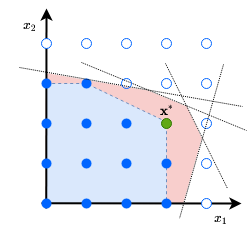
\includegraphics[width=0.45\textwidth]{../figure/valid_ineq.png}
		\caption{Illustration of valid inequalities\footnote{\tiny Módos, I. (2023, January 29). Mixed Integer Linear Programming: Introduction. Medium. https://towardsdatascience.com/mixed-integer-linear-programming-1-bc0ef201ee87
		}}
		\label{fig:sample-image}
	\end{figure}
\end{frame}

\subsection{valid inequalities for faster convergence}
\begin{frame}
	\begin{equation}
		\begin{aligned}
		&\begin{aligned}
		\min _{\alpha_j, \delta_j, \delta_j^2, \gamma_j^1, \gamma_j^2} \alpha_j & +\delta_j^1\left(\mu_j(y)+\epsilon_j^\mu\right)-\delta_j^2\left(\mu_j(y)-\epsilon_j^\mu\right)+\gamma_j^1\left(\sigma_j^2(y)\right. \\
		& \left.+\left(\mu_j(y)\right)^2\right) \bar{\epsilon}_j^\sigma-\gamma_j^2\left(\sigma_j^2(y)+\left(\mu_j(y)\right)^2\right) \underline{\epsilon}_j^\sigma
		\end{aligned}\\
		\text { s.t. } \quad &\alpha_j+\left(\delta_j^1-\delta_j^2\right) \xi_k+\left(\gamma_j^1-\gamma_j^2\right) \xi_k^2 \geq \theta_{j k}(y) \quad k=1, \ldots, K \text {, }\\
		&\delta_j^1, \gamma_j^1, \delta_j^2, \gamma_j^2 \geq 0
		\end{aligned}
		\end{equation}
\end{frame}

\subsection{Extreme Rays}
\begin{frame} Let:
	\begin{equation}
		\delta_j:=\delta_j^1-\delta_j^2 \text, \gamma_j:=\gamma_j^1-\gamma_j^2
	\end{equation}
	Problem's constraints are equivalent to:
	\begin{equation}
		\alpha_j+\delta_j \xi_k+\gamma_j \xi_k^2 \geq \theta_{j k}(y) \quad k=1, \ldots, K
		\end{equation}
	To identify extreme rays:
	\begin{equation}
		\begin{aligned}
		& \text{For arbitrary: } m, n \in\{1, \ldots, K\} \text{with: } \xi_m<\xi_n\\
		& \alpha_j+\delta_j \xi_m+\gamma_j \xi_m^2=0 \\
		& \alpha_j+\delta_j \xi_n+\gamma_j \xi_n^2=0 \\
		& \alpha_j+\delta_j \xi_k+\gamma_j \xi_k^2 \geq 0 \quad k \in\{1, \ldots, K\} \backslash\{m, n\}
		\end{aligned}
	\end{equation}
	Solution:
	\begin{equation}
		\begin{aligned}
		& \delta_j= -(\xi_m+\xi_n)\gamma_j \\
		& \alpha_j=\xi_m\xi_n\gamma_j\\
		\end{aligned}
	\end{equation}
\end{frame}	

\begin{frame} Let:
	\begin{equation}
		\begin{aligned}
		& \delta_j= -(\xi_m+\xi_n)\gamma_j \\
		& \alpha_j=\xi_m\xi_n\gamma_j\\
		\end{aligned}
	\end{equation}
	If $\gamma=1$:\\
	\quad$(\xi_k - \xi_m)(\xi_k-\xi_n)\geq0 \quad k \in\{1, \ldots, K\} \backslash\{m, n\}$\\
	\quad equivalent to :$\xi_k\geq\xi_m\text,\xi_k\geq\xi_n\quad\text{or}\quad\xi_k\leq\xi_m,\xi_k\leq\xi_n$\\
	Extreme rays generator:
	\begin{equation}
		\begin{aligned}
		& \left(\alpha_j, \delta_j, \gamma_j\right): \\
		& \cdot\left(\xi_{(1)} \xi_{(2)},-\left(\xi_{(1)}+\xi_{(2)}\right), 1\right) \\
		& \cdot\left(\xi_{(K-1)} \xi_{(K)},-\left(\xi_{(K-1)}+\xi_{(K)}\right), 1\right)
		\end{aligned}
	\end{equation}


	If $\gamma=-1$:\\
	\quad$(\xi_k - \xi_m)(\xi_k-\xi_n)\leq0 \quad k \in\{1, \ldots, K\} \backslash\{m, n\}$\\
	\quad equivalent to : $\xi_m\leq\xi_k\leq\xi_n$
	
	Extreme rays generator:\\
	\begin{equation}
		\left(-\xi_{(1)} \xi_{(K)}, \xi_{(1)}+\xi_{(K)},-1\right)
	\end{equation}
\end{frame}	

\subsection{Valid inequalities}
\begin{frame}
	\begin{equation}
		\begin{aligned}
		& \xi_{(1)} \xi_{(2)}-\left(\xi_{(1)}+\xi_{(2)}\right)\left(\mu_j(y)-\epsilon_j^\mu\right)+\left(\sigma_j^2(y)+\left(\mu_j(y)\right)^2\right) \bar{\epsilon}_j^\sigma \\
		& \geq 0 \quad \forall j \in J \\
		& \xi_{(K-1)} \xi_{(K)}-\left(\xi_{(K-1)}+\xi_{(K)}\right)\left(\mu_j(y)-\epsilon_j^\mu\right)+\left(\sigma_j^2(y)+\left(\mu_j(y)\right)^2\right) \bar{\epsilon}_j^\sigma \\
		& \geq 0 \quad \forall j \in J \\
		& -\xi_{(1)} \xi_{(K)}+\left(\xi_{(1)}+\xi_{(K)}\right)\left(\mu_j(y)+\epsilon_j^\mu\right)-\left(\sigma_j^2(y)+\left(\mu_j(y)\right)^2\right) \underline{\epsilon}_j^\sigma \\
		& \geq 0 \quad \forall j \in J
		\end{aligned}
	\end{equation}
\end{frame}	

\subsection{McCormick envelopes to linearize Valid inequalities}
\begin{frame}
	\begin{equation}
		\begin{aligned}
		&\xi_{(1)} \xi_{(2)}-\left(\xi_{(1)}+\xi_{(2)}\right)\left(\bar{\mu}_j\left(1+\sum_i \lambda_{j i}^\mu y_i\right)-\epsilon_j^\mu\right)+\Theta_j \bar{\epsilon}_j^\sigma \geq 0 \quad \forall j \in J
		& \xi_{(K-1)} \xi_{(K)}-\left(\xi_{(K-1)}+\xi_{(K)}\right)\left(\bar{\mu}_j\left(1+\sum_{i^{\prime} \in I} \lambda_{j i^{\prime}}^\mu y_{i^{\prime}}\right)-\epsilon_j^\mu\right)+\Theta_j \bar{\epsilon}_j^\sigma \\
		& \quad \geq 0 \quad \forall j \in J \\
		& -\xi_{(1)} \xi_{(K)}+\left(\xi_{(1)}+\xi_{(K)}\right)\left(\bar{\mu}_j\left(1+\sum_{i^{\prime} \in I} \lambda_{j i^{\prime}}^\mu y_{i^{\prime}}\right)+\epsilon_j^\mu\right)-\Theta_j \epsilon_j^\sigma \\
		& \quad \geq 0 \quad \forall j \in J \\
		& \Theta_j=\bar{\sigma}_j^2+\bar{\mu}_j^2+\sum_{i^{\prime} \in I} \Lambda_{j i^{\prime}} y_{i^{\prime}}+2 \bar{\mu}_j^2 \sum_{l=1}^{|l|} \sum_{m=1}^{l-1} \lambda_{j l}^\mu \lambda_{j m}^\mu Y_{l m} \quad \forall j \in J \\
		& \left(Y_{l m}, y_l, y_m\right) \in M_{(0,1)}^{\prime} \quad \forall l=1, \ldots,|I|, l>m .
		\end{aligned}
	\end{equation}
\end{frame}	

\section{Experiments} % Mohammad ~ 3 min.
\begin{frame}[allowframebreaks]
	We compare three solvers: \texttt{BASSolver}, \texttt{DRSOlver} and \texttt{PSolver}.
	\begin{columns}
		\column{0.5\textwidth}
		\begin{itemize}
			\item $I = 10$ and $J = 20$
			\item $\Dcal = [100]$
			\item Opening costs $\sim U(5000, 10000)$
			\item Transportation fees $\propto L_2$-distance
			\item Capacities $\sim U(10, 20)$
			\item Revenue fixed to 150
			\item Penalty fixed to 225
		\end{itemize}
		
		\column{0.7\textwidth}
		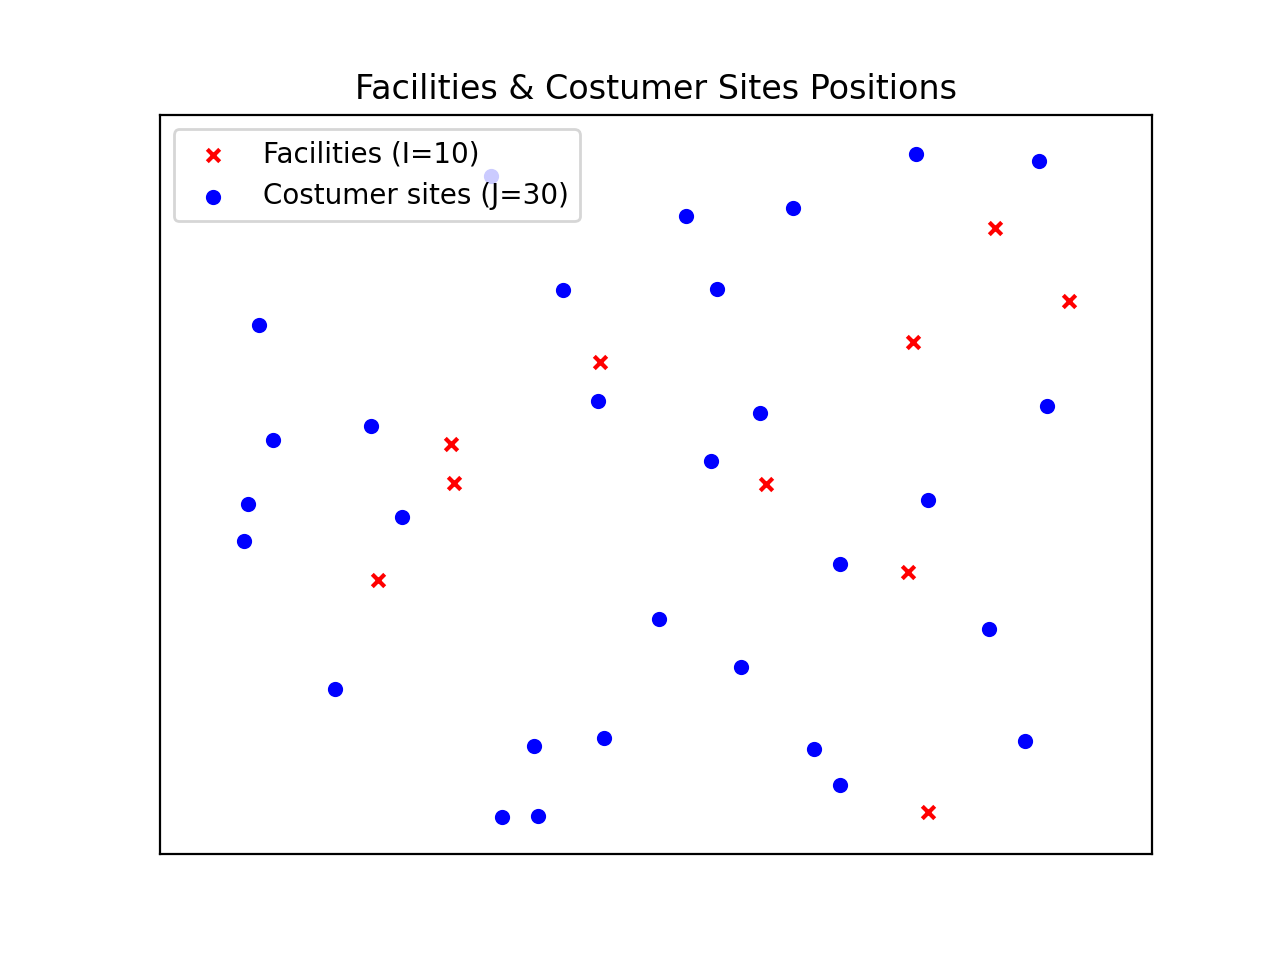
\includegraphics[width=\textwidth]{../figure/facility_costumer_site_pos.png}
	\end{columns}
	
	\framebreak
	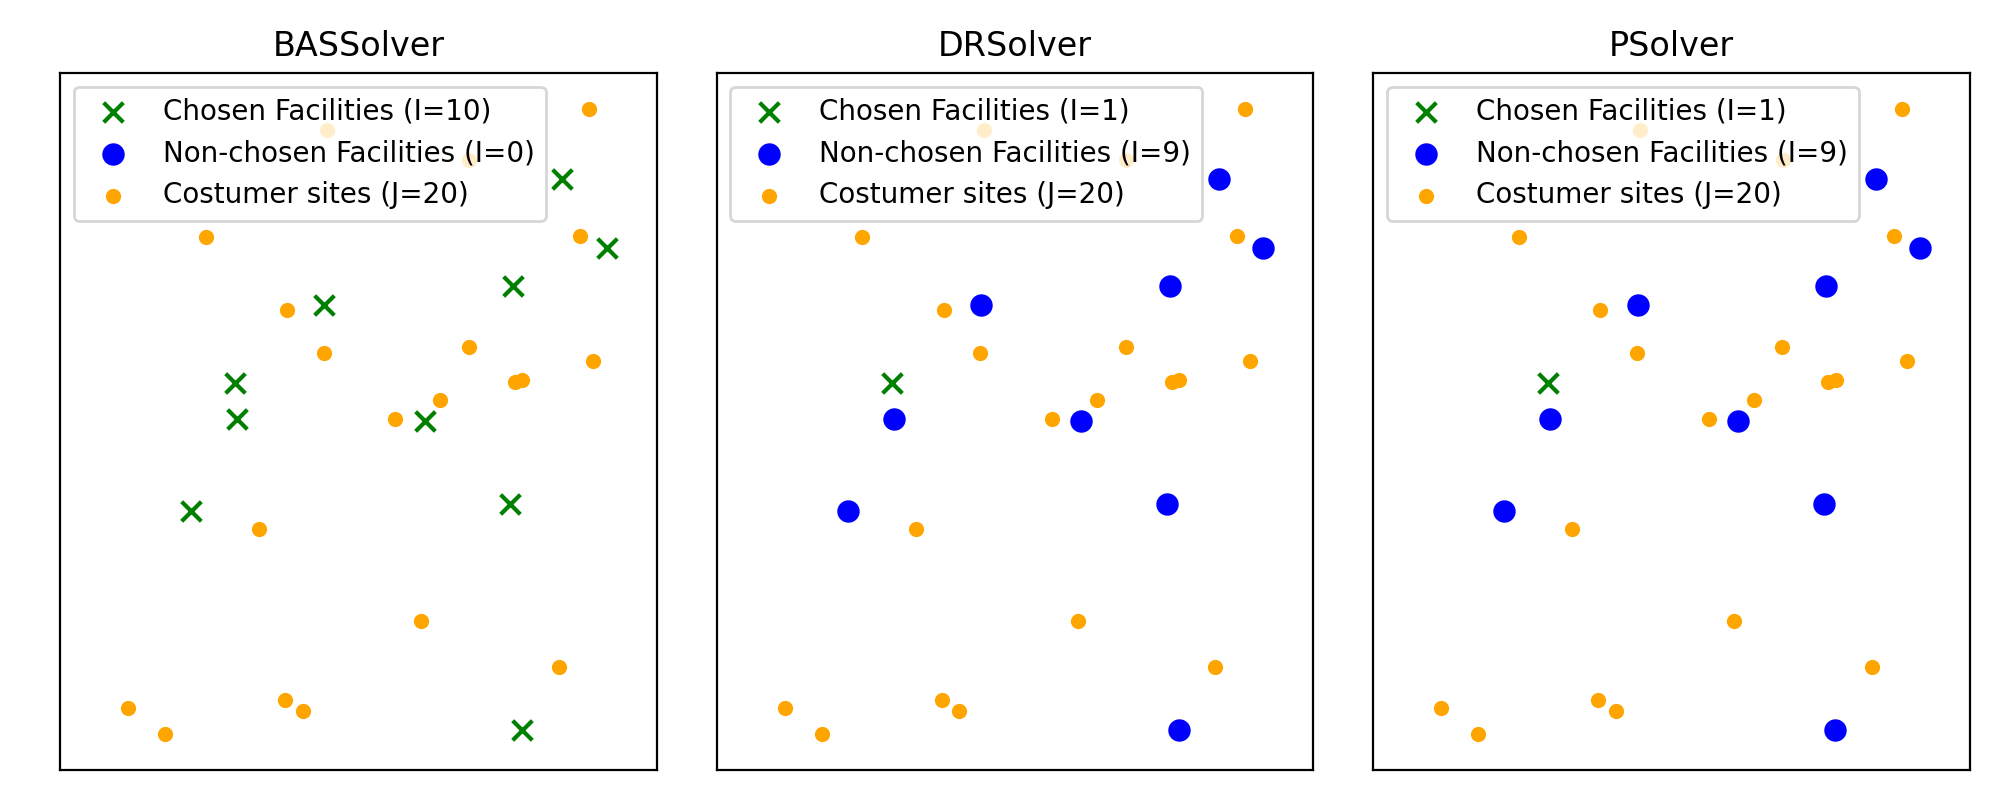
\includegraphics[width=\textwidth]{../figure/chosen_facility_costumer_site_pos.png}
	
	\framebreak
	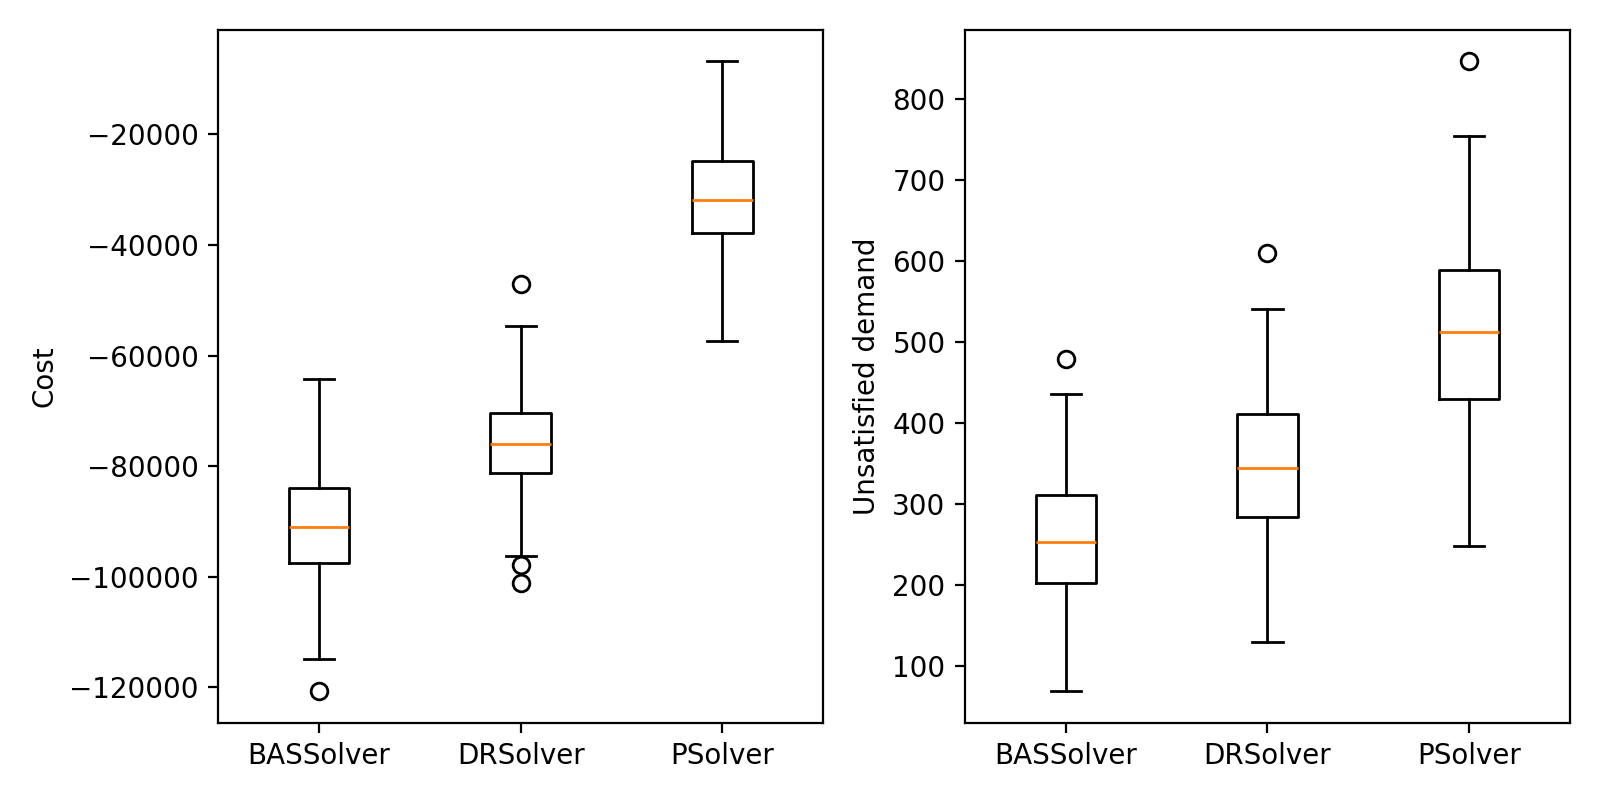
\includegraphics[width=\textwidth]{../figure/benchmark.png}
\end{frame}

%\section{What more?} % ~ Mohammad 3 min.
%\begin{frame}
	% TODO: Present the improvments to come
%\end{frame}
\end{document}